\documentclass[letterpaper]{report}
\usepackage[letterpaper, total={4.5in,8.5in}]{geometry}
\usepackage{merriweather}
\usepackage[T1]{fontenc}
\usepackage{graphicx}
\usepackage{float}
\usepackage{subcaption}
\graphicspath{.}
\title{A Tight, Incremental Movement Shooter}
\author{Thamsen Borges}
\date{\today}
\begin{document}
\maketitle
% \part \chapter \section \subsection \paragraph \subparagraph
\part{Introduction}
	\chapter{Project Parameters}
		\section{Primary Design Technique}
			For the development of this prototype, I selected a whitebox approach--paper prototyping didn't allow for exploring the sense of scale that I wanted to use to direct the player's mood, so a 3D approach was necessary to iterate on.
		\section{Camera System}
			I selected a first person camera system to complement the above; by allowing the player to sweep their view through space as if they were there, they can appreciate the mood change when that space is personally encroached, and it also allows for better control of the later grappling mechanic.
		\section{Game Rules}
			\subsection{Overview}
				\paragraph{Systems}
					\subparagraph{"Health"}
						When the player is contacted by an enemy, a death animation plays, and the level is restarted.
					\subparagraph{Physics}
						The player moves through a space with gravity and collision, and jumping/grappling have similar feelings to what would happen if the player did the same thing on Earth.
					\subparagraph{Weaponry}
						The player possesses items that fire when the mouse is clicked and interact with the world in various ways (see the next subsection for details).
			\subsection{Weapons}
				\paragraph{Pistol}
					For the beginning weapon, a pistol, similar to the Sidekick from \emph{Halo: Combat Evolved}, was selected, as I wanted to enforce a feeling of the player's relative struggle in the situation, motivating them to keep moving to hopefully relieve the building tension of the first level.
				\paragraph{Grappling Hook}
					After the first level, the tension is released into a much faster pace, in which the player must escape an enclosing threat. To ratchet up the pace, the player is given a grapple hook, similar to Pathfinder's in \emph{Apex Legends}, in which the player can aim, fire, and latch on to scenery, using their momentum to propel them through the air.
				\paragraph{Antibody Gun}
					At the end of the emotional ramp, to ratchet up the stakes from "panic" to "frenzy," the player is given a weapon that can devastate and destroy the previous threats that forced them to flee. This weapon rips through both enemies and enemy-generated terrain, allowing the player to traverse the landscape back to the boss.
		\section{Narrative}
			\subsection{A citizen on a long city street is the only one that can help an outbreak}
				\paragraph{No Way Out} The player is dropped cold onto a street with a pistol in front of them. The approaching enemies, all from one direction, with no way out for the player, calls them to advance down the street to the source.
				\paragraph{Escape} As they arrive at the monolithic building that seems to be the source of the problem, they discover a powered grappling hook just before enormous, corrupt tendrils erupt from the building and start spreading across the city. The biomass starts to seal the player off, and they're forced to flee by swinging through the city, as they see something in the distance dropped from a space pod.
				\paragraph{Return} When they reach the drop point, they discover the Antibody Gun, a weapon that allows them to churn through the accumulated biomass and enemies with ease, still able to use their grappling hook to quickly return and destroy the Source.

\part{Game Design}
	\section{Core Mechanics}
		\subsection{Standard FPS actions}
			\paragraph{Look} The player can move the mouse to look around the environment.
			\paragraph{Move} WASD (or controller equivalents) can be used to move forward, backward, and sideward.
			\paragraph{Jump} Spacebar (or controller "A" equivalent) can be used to jump in a parabolic arc in a realistic manner.
			\paragraph{Shoot} The left mousebutton (or right trigger on a controller) can be used to shoot the active weapon.
	\section{Gameplay Loop Diagram}
		\begin{figure}[h!]
			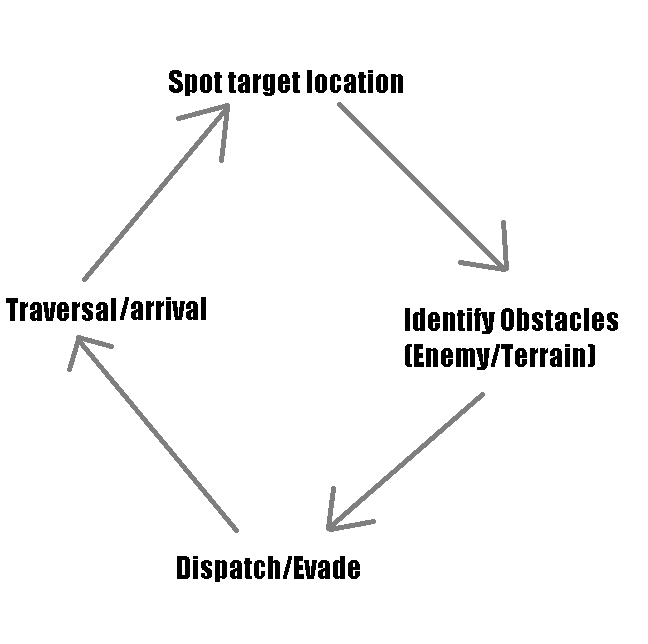
\includegraphics[scale=.5]{loop}
		\end{figure}
	\section{Movement and abilities}
		\paragraph{See Above} The primary movement techniques remain the same until Level Two, where the grappling hook is acquired. After that, the main augmentation is the ability to:
		\paragraph{Swing} After grappling an object, the player can use their movement keys to modify the arc of their swing, and the grappling button can be released to course through the air for either a landing or a re-grapple.

\part{Three Levels}
	\chapter{Level One}
		\section{Design goals}
			\subsection{Establish World}
			\subsection{Familiarize Player}
			\subsection{Build Tension}
		\section{Narrative}
			\paragraph{Beginning} The player is thrust into a mid-day city street with a pistol in front of them. In the distance looms a large, monolithic building, and in between that and them are slightly corrupt, slow-moving enemies. With no way out but through, the player must continue toward this large eyecatch while evading enemies that are only immobilized or hindered by the pistol's gunfire.
			\paragraph{Middle} It becomes more and more obvious as the player continues that the source of these entities is the building in the distance, as the traversal toward it becomes more obscured by them.
			\paragraph{End} Once the final corridor is easy to see through, another "weapon" is visible through the thin corridor, right in front of the entrance to this large structure--finally, the player has reached the destination, but something else is amiss.
			
		\section{Aesthetic}
			\paragraph{An interrupted cityscape} The bright reflections off of large, glassy buildings around them is currently only contrasted by the disturbed-looking entities walking through this street. The balance of cramped and open is apparent in the middle of this street.
			
			\subsection{Imagery}
				\begin{figure}[H]
					\begin{subfigure}[h]{.32\linewidth}
						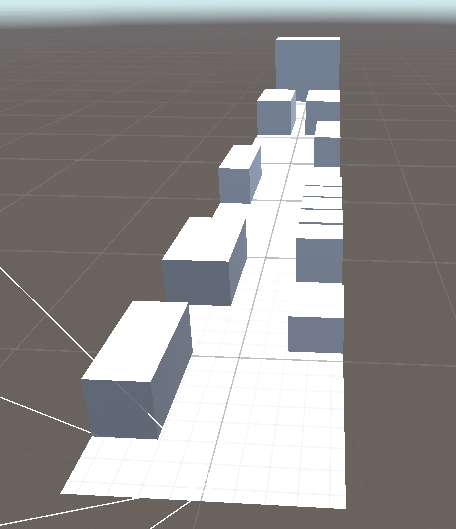
\includegraphics[width=\linewidth]{level1-1}
					\end{subfigure}
					\begin{subfigure}[h]{.32\linewidth}
						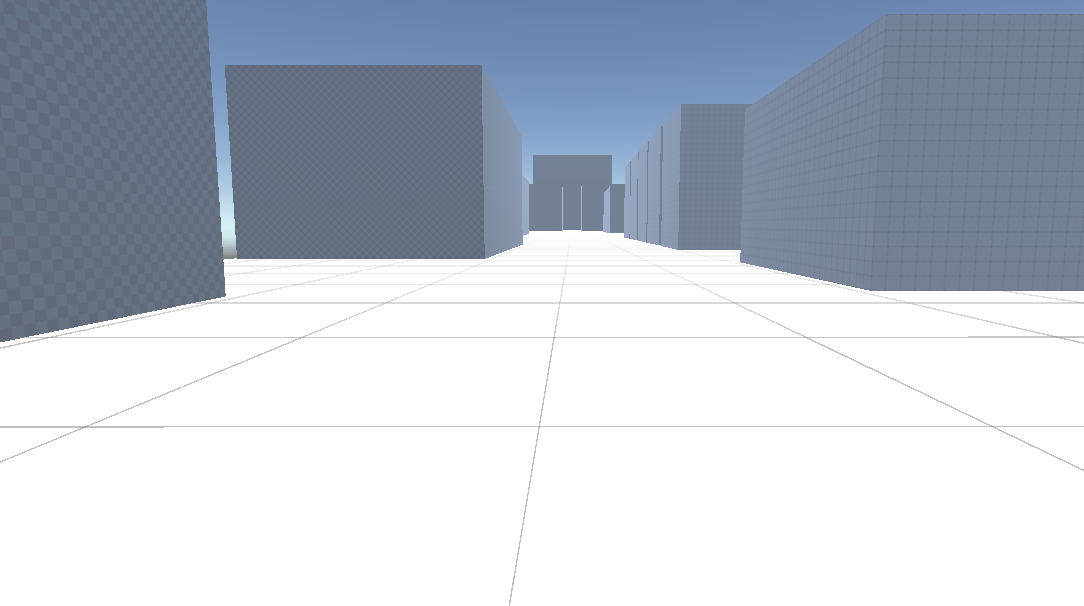
\includegraphics[width=\linewidth]{level1-2}
					\end{subfigure}
					\begin{subfigure}[h]{.32\linewidth}
						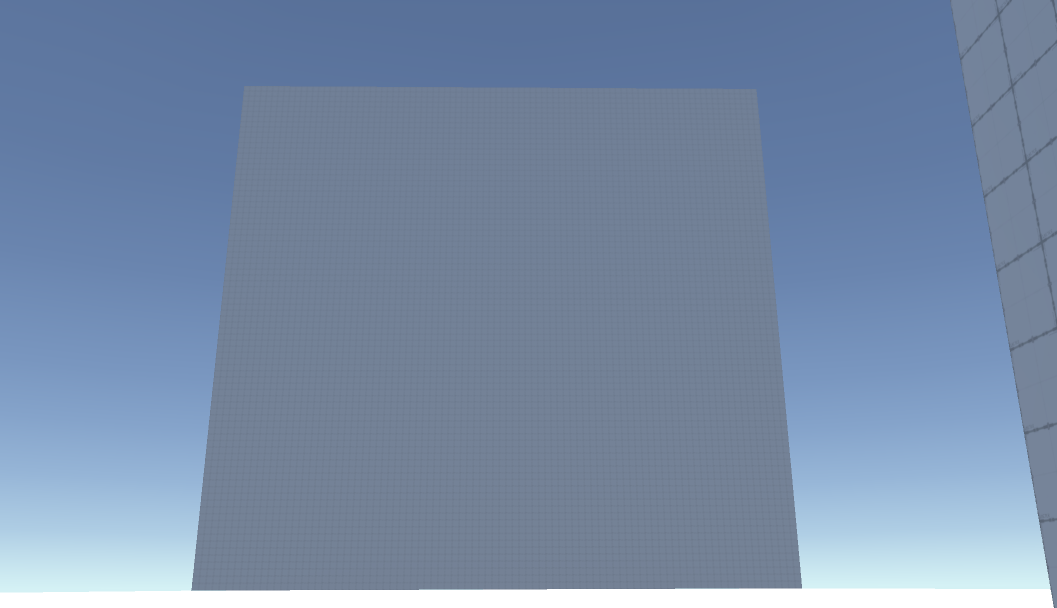
\includegraphics[width=\linewidth]{level1-3}
					\end{subfigure}
				\end{figure}
				
			\subsection{Audio}
				\paragraph{The Division - Sampled Soundscape} The loudness of the footsteps, the openness of the soundscape, and the progressively louder wind captures the same idea that will be used in this ramp-level. \\ https://www.youtube.com/watch?v=f974gB-EYy\&t=4616s
				
	\chapter{Level Two}
		\section{Design Goals}
			\subsection{Leverage tension and attention to up the ante}
			\subsection{Immerse player in swinging/navigation mechanic}
			\subsection{Build player's anticipation of next level (the weapon drop)}
		\section{Narrative}
			\paragraph{Beginning} What seemed disturbed before is now clearly pissed off. After the player grabs the grappling hook, the building's upper levels emit a thunderous rumble as enormous tendrils blast out of the walls, churning through the landscape. Simultaneously, biomass accumulates between the two tendrils and the surrounding structures, entrapping the player if they're not quick enough to leave.
			\paragraph{Middle} The tendrils continue coursing through the street, and the player follows in tow. As they cross through the center point, a large drop pod comes from the sky, hurtling toward where the player began in level one.
			\paragraph{End} As they narrowly arrive at the drop pod, the tendrils burrow into the ground around it as the pod opens.
		\section{Aesthetic}
			\subsection{Enclosing corruption, navigating the large city, urgency, intensity}
			\subsection{Imagery}
				\begin{figure}[H]
					\begin{subfigure}[h]{.32\linewidth}
						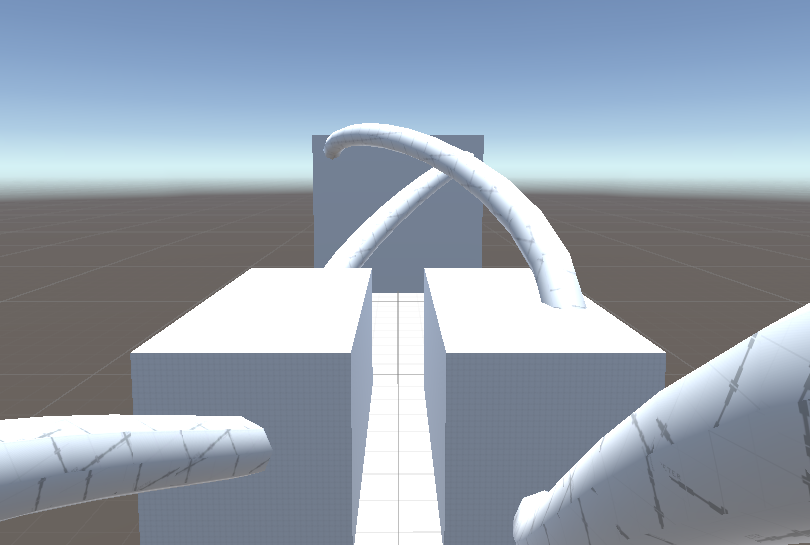
\includegraphics[width=\linewidth]{level2-1}
					\end{subfigure}
					\begin{subfigure}[h]{.32\linewidth}
						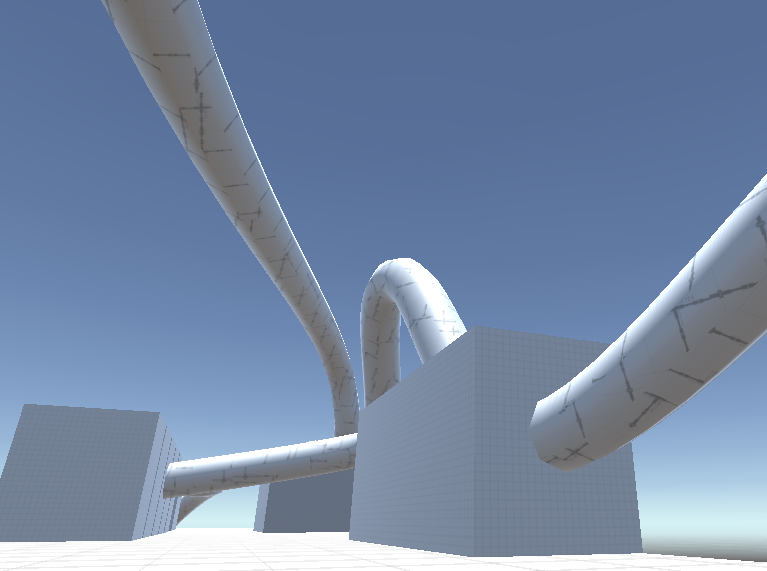
\includegraphics[width=\linewidth]{level2-2}
					\end{subfigure}
					\begin{subfigure}[h]{.32\linewidth}
						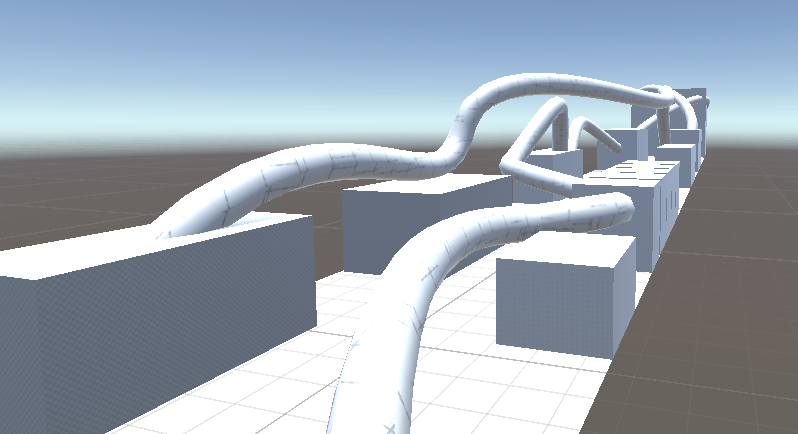
\includegraphics[width=\linewidth]{level2-3}
					\end{subfigure}
				\end{figure}
			\subsection{Audio}
				\paragraph{Oil Derrick Scene - There Will Be Blood} This overwhelming cacophony of various percussion instruments is perfectly paired to a scene where oil bursts forth from the earth in a demonstration of inhuman scales. The same feeling will be needed to keep the player aware of the stakes at hand. \\
				https://www.youtube.com/watch?v=oueJ\_eZ3yOY (Music starts at 1:30)
				
	\chapter{Level Three}
		\section{Design Goals}
			\subsection{Unleash player/enter "Frenzy" with powerful weapon}
			\subsection{Get player back to boss}
			\subsection{Transform expansive feeling to "enclosed" one}
		\section{Narrative}
			\paragraph{Beginning} The drop pod opens up to reveal the Antibody Gun, capable of destroying the ever-encroaching biomass and the enemies that are coming forth from it. It rends the flesh of the corruption apart, allowing the player to head back to where this all started.
			\paragraph{Middle} The carnage continues as the enemies become more numerous but equally weak, allowing the player to course through them with near impunity.
			\paragraph{End} Upon reaching the source, the player deals the final blows to the primary biomass that has been centralized in this space, finally dismantling this wretched infestation.
		\section{Aesthetic}
			\subsection{Frenzy through dingy corruption and gloom within corrupted caverns, lit by the Antibody Gun's reactions with the flesh, progressively "cleansed"}
			\subsection{Imagery}
				\begin{figure}[H]
					\begin{subfigure}[h]{.32\linewidth}
					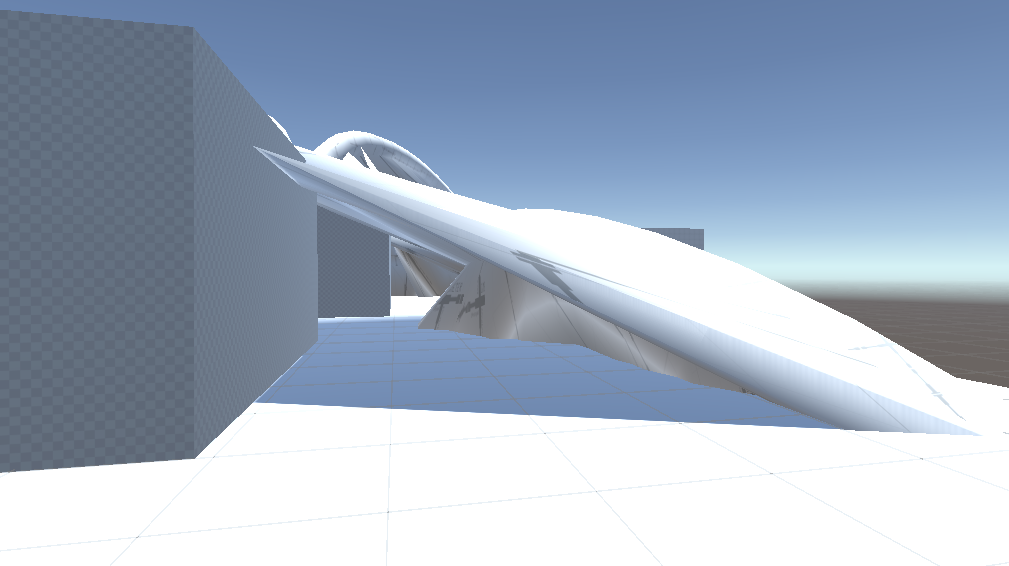
\includegraphics[width=\linewidth]{level3-1}
					\end{subfigure}
					\begin{subfigure}[h]{.32\linewidth}
					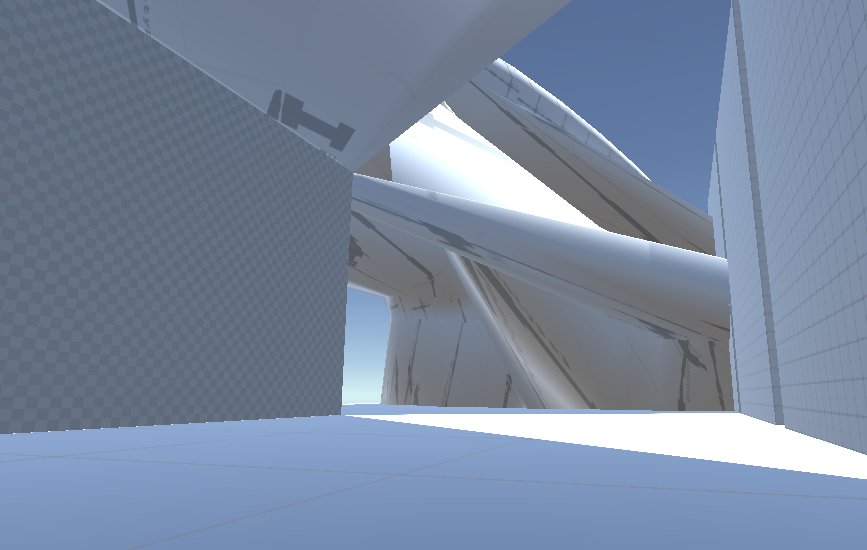
\includegraphics[width=\linewidth]{level3-2}
					\end{subfigure}
					\begin{subfigure}[h]{.32\linewidth}
					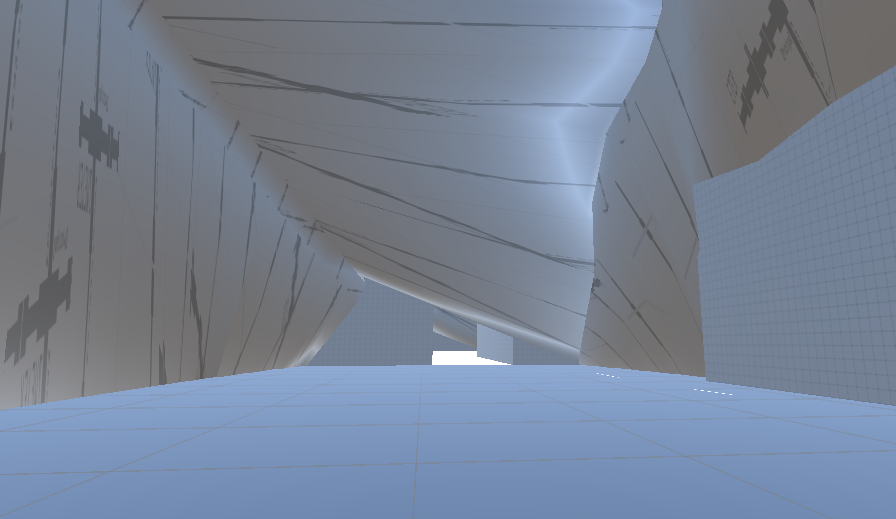
\includegraphics[width=\linewidth]{level3-3}
					\end{subfigure}
				\end{figure}
			\subsection{Audio}
				\paragraph{Mick Gordon's "BFG Division"} It's on the nose, but this best represents the feeling of finally obliterating the encroaching threat. Link for reference (The music played during this section would be similar): \\ https://www.youtube.com/watch?v=QHRuTYtSbJQ
			
\end{document}